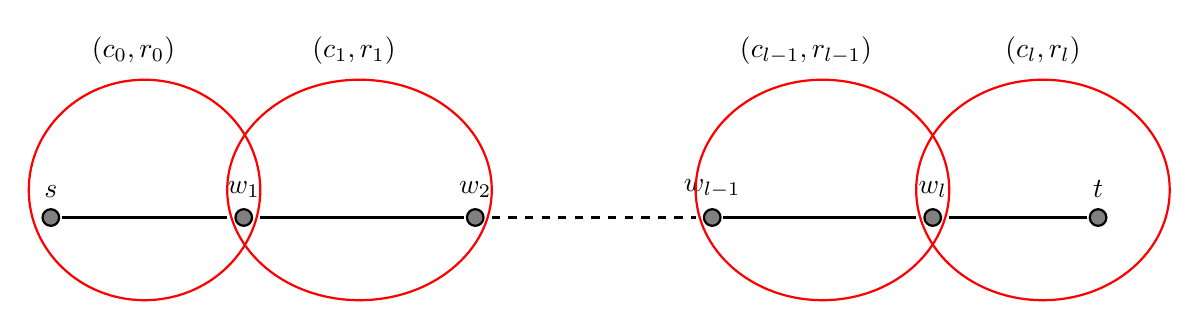
\begin{tikzpicture}[thick,scale=0.7]
	\draw (0, 0) node[circle, draw, fill=black!50, inner sep=0pt, minimum width=6pt, label = $s$] {};
	\draw (19, 0) node[circle, draw, fill=black!50, inner sep=0pt, minimum width=6pt,label = $t$] {};
	
	\draw (3.5, 0) node[circle, draw, fill=black!50, inner sep=0pt, minimum width=6pt,label = $w_1$] {};
	\draw [line width = 0.5mm] (0.2, 0) -- (3.2, 0);
	\draw [red] (1.7, 0.5) ellipse (2.1 and 2);
	\draw (1.5, 2.4) node[red, label={$\ball(c_0, r_{0})$}]{};
	
	\draw (7.7, 0) node[circle, draw, fill=black!50, inner sep=0pt, minimum width=6pt,label = $w_2$] {};
	\draw [line width = 0.5mm] (3.8, 0) -- (7.5, 0);
	\draw [red] (5.6, 0.5) ellipse (2.4 and 2);
	\draw (5.5, 2.4) node[red, label={$\ball(c_1, r_{1})$}]{};
	
	\draw (16, 0) node[circle, draw, fill=black!50, inner sep=0pt, minimum width=6pt,label = $w_l$] {};
	\draw [line width = 0.5mm] (18.8, 0) -- (16.3, 0);
	\draw [red] (18, 0.5) ellipse (2.3 and 2);
	\draw (18, 2.4) node[red, label={$\ball(c_{l}, r_{l})$}]{};
	
	\draw (12, 0) node[circle, draw, fill=black!50, inner sep=0pt, minimum width=6pt,label = $w_{l-1}$] {};
	\draw [line width = 0.5mm] (15.7, 0) -- (12.2, 0);
	\draw [red] (14, 0.5) ellipse (2.3 and 2);
	\draw (13.7, 2.4) node[red, label={$\ball(c_{l-1}, r_{l-1})$}]{};
	
	\draw [dashed] (8, 0) -- (11.7, 0); 
\end{tikzpicture}